\chapter{Méthodologie}
\label{chap:methodologie}

\section{Description du dataset}

\subsection{Caractéristiques générales}

Le dataset BRFSS (\textit{Behavioral Risk Factor Surveillance System}) 2020--2024 poolé et préparé pour le machine learning présente les caractéristiques décrites dans le tableau \ref{tab:dataset_chars}.

\begin{table}[H]
\centering
\caption{Caractéristiques du dataset BRFSS 2020--2024}
\label{tab:dataset_chars}
\begin{tabular}{ll}
\toprule
\textbf{Caractéristique} & \textbf{Valeur} \\
\midrule
Nombre d'observations brutes & 2\,176\,776 \\
Doublons supprimés & 416\,535 \\
Nombre d'observations après nettoyage & 1\,760\,241 \\
Nombre de variables modélisées & 14 (+ 2 features dérivées) \\
Variable cible & \texttt{HeartDiseaseorAttack} (binaire, 0/1) \\
Prévalence MCV (classe positive) & 10,32\% \\
Format source & Parquet (fichier poolé \texttt{\_ml}) \\
\bottomrule
\end{tabular}
\end{table}

\subsection{Variables sélectionnées}

Les 14 variables retenues après sélection sont décrites dans le tableau \ref{tab:variables}. Ces variables ont été choisies parmi les 129 colonnes du dataset brut BRFSS sur la base de leur pertinence clinique documentée dans la littérature et de leur disponibilité dans le fichier poolé ML.

\begin{longtable}{p{3.8cm}p{4cm}p{2cm}p{3.5cm}}
\caption{Variables sélectionnées et leur encodage}
\label{tab:variables}\\
\toprule
\textbf{Variable} & \textbf{Description} & \textbf{Type} & \textbf{Encodage} \\
\midrule
\endfirsthead
\multicolumn{4}{c}{\textit{Suite du tableau \ref{tab:variables}}}\\
\toprule
\textbf{Variable} & \textbf{Description} & \textbf{Type} & \textbf{Encodage} \\
\midrule
\endhead
\bottomrule
\endlastfoot
\texttt{HeartDiseaseorAttack} & Maladie coronarienne ou IM & Binaire & 0=Non, 1=Oui \\
\texttt{BMI} & Indice de masse corporelle & Continu & \_BMI5 / 100 \\
\texttt{Smoker} & Tabagisme (100+ cigarettes/vie) & Binaire & 0=Non, 1=Oui \\
\texttt{Stroke} & Antécédent d'AVC & Binaire & 0=Non, 1=Oui \\
\texttt{Diabetes} & Diabète diagnostiqué & Binaire & 0=Non, 1=Oui \\
\texttt{PhysActivity} & Activité physique (30j) & Binaire & 0=Non, 1=Oui \\
\texttt{GenHlth} & Santé générale auto-évaluée & Ordinal & 1=Excellent à 5=Mauvaise \\
\texttt{MentHlth} & Jours santé mentale mauvaise & Discret & 0--30 jours (88→0) \\
\texttt{PhysHlth} & Jours santé physique mauvaise & Discret & 0--30 jours \\
\texttt{DiffWalk} & Difficultés à marcher & Binaire & 0=Non, 1=Oui \\
\texttt{Sex} & Sexe & Binaire & 0=Homme, 1=Femme \\
\texttt{Age} & Tranche d'âge BRFSS & Ordinal & 1 (18-24) à 13 (80+) \\
\texttt{Education} & Niveau d'éducation & Ordinal & 1 (aucune) à 6 (diplômé) \\
\texttt{HvyAlcoholConsump} & Consommation excessive d'alcool & Binaire & 0=Non, 1=Oui \\
\bottomrule
\end{longtable}

\subsection{Variables absentes du fichier poolé ML}

Une contrainte importante de ce travail est l'absence de quatre variables cliniquement importantes dans le fichier poolé ML disponible :

\begin{itemize}
    \item \texttt{HighBP} (hypertension artérielle) — remplacée par \texttt{Stroke} dans le calcul du RiskScore
    \item \texttt{HighChol} (hypercholestérolémie) — remplacée par \texttt{DiffWalk} dans le calcul du RiskScore
    \item \texttt{Income} (revenu du foyer) — absente du modèle
    \item \texttt{NoDocbcCost} (renoncement aux soins pour raisons financières) — absente du modèle
\end{itemize}

Ces variables, présentes dans le fichier EDA et abondamment utilisées dans la littérature (Nickels et al.\ obtiennent une AUC de 0,912 avec \texttt{HighBP}/\texttt{HighChol}), expliquent en partie le plateau d'AUC observé à 0,82 dans nos modèles. Cette limitation est d'ordre documentaire et non algorithmique.

% ─────────────────────────────────────────────────────────────────────────────
\section{Architecture du pipeline}
% ─────────────────────────────────────────────────────────────────────────────

Le pipeline développé dans ce projet suit une architecture séquentielle en cinq phases, représentée à la figure~\ref{fig:pipeline}. Chaque phase produit des artefacts persistants — fichiers au format Parquet, tableaux NumPy, fichiers JSON — qui constituent les entrées de la phase suivante, garantissant la reproductibilité de l'ensemble du processus et facilitant la reprise en cas d'interruption de session.

\begin{figure}[H]
\centering
\begin{tikzpicture}[
    box/.style={rectangle, draw=primary, fill=primary!10, rounded corners=5pt,
                minimum width=11cm, minimum height=1.1cm,
                text centered, font=\small\bfseries, text=primary!85!black},
    arr/.style={->, >=stealth, thick, color=primary}
]
    \node[box] at (0, 0)   (p1)
        {Phase 1 — Ingestion et nettoyage
         {\normalfont\scriptsize\itshape (PySpark, Parquet, binarisation BRFSS, déduplication)}};
    \node[box] at (0,-1.9) (p2)
        {Phase 2 — Analyse exploratoire et Feature Engineering
         {\normalfont\scriptsize\itshape (corrélation, Gini, $\chi^2$, ACP, features dérivées)}};
    \node[box] at (0,-3.8) (p3)
        {Phase 3 — Entraînement du réseau de neurones profond
         {\normalfont\scriptsize\itshape (TensorFlow/Keras, class weights, optimisation du seuil)}};
    \node[box] at (0,-5.7) (p4)
        {Phase 4 — Entraînement XGBoost et Spark GBT
         {\normalfont\scriptsize\itshape (RandomizedSearchCV, benchmark distribué)}};
    \node[box] at (0,-7.6) (p5)
        {Phase 5 — Évaluation comparative et visualisation
         {\normalfont\scriptsize\itshape (métriques, courbes ROC, dashboard Streamlit)}};
    \draw[arr] (p1.south) -- (p2.north);
    \draw[arr] (p2.south) -- (p3.north);
    \draw[arr] (p3.south) -- (p4.north);
    \draw[arr] (p4.south) -- (p5.north);
\end{tikzpicture}
\caption{Architecture du pipeline Big Data en cinq phases séquentielles}
\label{fig:pipeline}
\end{figure}

\begin{enumerate}
    \item \textbf{Phase 1 — Ingestion et nettoyage} : Chargement du fichier Parquet (2\,176\,776 lignes) avec PySpark en mode distribué, application du pipeline de binarisation BRFSS, suppression des enregistrements dupliqués et imputation des valeurs manquantes. Le jeu de données résultant compte 1\,760\,241 observations.

    \item \textbf{Phase 2 — Analyse exploratoire et Feature Engineering} : Calcul des matrices de corrélation (Pearson, Spearman), évaluation de l'importance prédictive par la réduction d'impureté de Gini et le test du $\chi^2$, analyse en composantes principales, et construction de deux variables composites (RiskScore, HealthIndex). Le jeu de données final comprend 15 features sélectionnées.

    \item \textbf{Phase 3 — Entraînement du DNN} : Partitionnement stratifié 70/15/15, normalisation par StandardScaler, entraînement du réseau de neurones profond avec gestion du déséquilibre de classes par pondération explicite et protocole de régularisation (Dropout, BatchNormalization, régularisation $L_2$), puis optimisation du seuil de classification par courbe Précision-Rappel.

    \item \textbf{Phase 4 — Entraînement XGBoost et Spark GBT} : Optimisation des hyperparamètres d'XGBoost par RandomizedSearchCV (validation croisée 3-fold), entraînement du GBTClassifier de Spark MLlib sur les données complètes, et benchmark contrôlé des temps d'entraînement sur cinq fractions croissantes du jeu de données.

    \item \textbf{Phase 5 — Évaluation comparative et visualisation} : Calcul des métriques d'évaluation (accuracy, précision, rappel, F1-score, AUC-ROC) sur le même jeu de test pour les trois modèles, génération des courbes ROC et matrices de confusion, et déploiement d'un tableau de bord interactif Streamlit.
\end{enumerate}

% ─────────────────────────────────────────────────────────────────────────────
\section{Prétraitement des données}
% ─────────────────────────────────────────────────────────────────────────────

\subsection{Binarisation spécifique au format BRFSS}

Le format BRFSS utilise des conventions d'encodage spécifiques qui diffèrent des standards numériques attendus par les algorithmes de machine learning. Les variables dichotomiques suivent la convention $1 = \text{Oui}$, $2 = \text{Non}$ — à l'inverse du schéma binaire $\{0, 1\}$ standard. Une étape de binarisation explicite est donc appliquée en priorité sur l'ensemble du jeu de données selon le schéma général :

\begin{equation}
x_{\text{binaire}} = \begin{cases}
1 & \text{si valeur BRFSS} = 1 \text{ (Oui)} \\
0 & \text{si valeur BRFSS} = 2 \text{ (Non)} \\
\text{NaN} & \text{sinon (valeur manquante ou refus de répondre)}
\end{cases}
\label{eq:binarisation}
\end{equation}

Trois variables nécessitent un traitement spécifique supplémentaire :

\begin{itemize}
    \item \textbf{Variable cible \texttt{HeartDiseaseorAttack}} : dérivée de la variable composite \texttt{\_MICHD}, calculée par le CDC comme l'union logique de la cardiopathie coronarienne (\texttt{CVDCRHD4}) et de l'infarctus du myocarde (\texttt{CVDINFR4}). Cette variable composite présente une prévalence de 10,32\%, cohérente avec les estimations épidémiologiques américaines. La variable \texttt{HAS\_HEART\_ATTACK} du fichier poolé ne couvre que les infarctus (prévalence de 5,51\%) et a donc été écartée.

    \item \textbf{Indice de masse corporelle (BMI)} : stocké en centièmes dans la variable brute \texttt{\_BMI5} par le CDC (par exemple, 2800 $\to$ 28,00~kg/m²), la conversion par division par 100 restitue la valeur physique réelle.

    \item \textbf{Santé mentale (MentHlth)} : le code BRFSS 88 signifie « aucun mauvais jour » et est converti en 0~; les valeurs en dehors de l'intervalle $[0, 30]$ sont traitées comme manquantes.
\end{itemize}

Ce pipeline de binarisation garantit la cohérence sémantique des données tout en les rendant compatibles avec les conventions numériques des bibliothèques de machine learning, avant tout calcul statistique ou entraînement de modèle.

\subsection{Gestion des doublons}

La déduplication est effectuée avec PySpark sur l'ensemble des 14 colonnes sélectionnées. Le dataset passe de 2\,176\,776 à 1\,760\,241 lignes après suppression de 416\,535 doublons (19,1\% du dataset brut). Ces doublons proviennent du regroupement de cinq années d'enquête BRFSS~: un même répondant peut figurer plusieurs années consécutives avec des réponses identiques sur les dimensions retenues. L'analyse de la composition des doublons révèle qu'ils proviennent à 98,5\% de la classe négative (non-MCV), ce qui fait passer la prévalence de la classe positive de 8,63\% (avant déduplication) à 10,32\% (après).

\subsection{Imputation des valeurs manquantes}

L'imputation est réalisée après binarisation, garantissant la cohérence des valeurs imputées avec les conventions numériques du pipeline :

\begin{itemize}
    \item \textbf{Variables continues} (BMI, MentHlth, PhysHlth) : imputation par la médiane, robuste aux distributions asymétriques et aux valeurs extrêmes. Les médianes obtenues sont respectivement 27,71~kg/m², 0~jour et 0~jour.
    \item \textbf{Variables ordinales et binaires} : imputation par le mode (valeur la plus fréquente). La variable \texttt{HvyAlcoholConsump} présente 53,32\% de valeurs manquantes~: ce module est optionnel dans le questionnaire BRFSS et n'a pas été collecté chaque année~; son mode (0, absence de binge drinking) est utilisé pour l'imputation.
\end{itemize}

\subsection{Gestion du déséquilibre de classes}

Le jeu de données nettoyé présente un déséquilibre significatif~: la classe positive (MCV diagnostiquée) représente 10,32\% des observations, soit un rapport de classe de 8,68~:~1. Ce déséquilibre est inhérent à la nature épidémiologique des données et reflète la prévalence réelle des maladies cardiovasculaires dans la population américaine adulte.

Sans traitement explicite, les classifieurs standard maximisent l'accuracy globale en prédisant systématiquement la classe majoritaire, ce qui les rend cliniquement inutiles. Deux grandes stratégies sont documentées dans la littérature pour remédier à ce problème~:

\begin{itemize}
    \item \textbf{Sur-échantillonnage synthétique (SMOTE)} \cite{chawla2002smote}~: génère des exemples synthétiques de la classe minoritaire par interpolation convexe entre exemples voisins dans l'espace des features. Cette approche augmente la taille de l'ensemble d'entraînement mais modifie les distributions statistiques originales et peut introduire du bruit cliniquement non interprétable.

    \item \textbf{Pondération de classes (\textit{class weights})}~: modifie la fonction de perte pour pénaliser davantage les erreurs sur la classe minoritaire, sans altérer les données elles-mêmes. Cette approche est retenue dans ce travail car elle préserve les distributions épidémiologiques originales, essentielles pour l'interprétabilité médicale, et est directement supportée par TensorFlow et XGBoost.
\end{itemize}

Les poids sont calculés selon la méthode \textit{balanced}, inversement proportionnels à la fréquence de chaque classe~:
\begin{equation}
w_k = \frac{N_{\text{total}}}{n_{\text{classes}} \times N_k}
\end{equation}

On obtient $w_0 = 0{,}558$ pour la classe négative et $w_1 = 4{,}847$ pour la classe positive. Pour XGBoost, le paramètre équivalent \texttt{scale\_pos\_weight} est fixé à $n_{\text{neg}}/n_{\text{pos}} \approx 8{,}69$.

\begin{figure}[H]
    \centering
    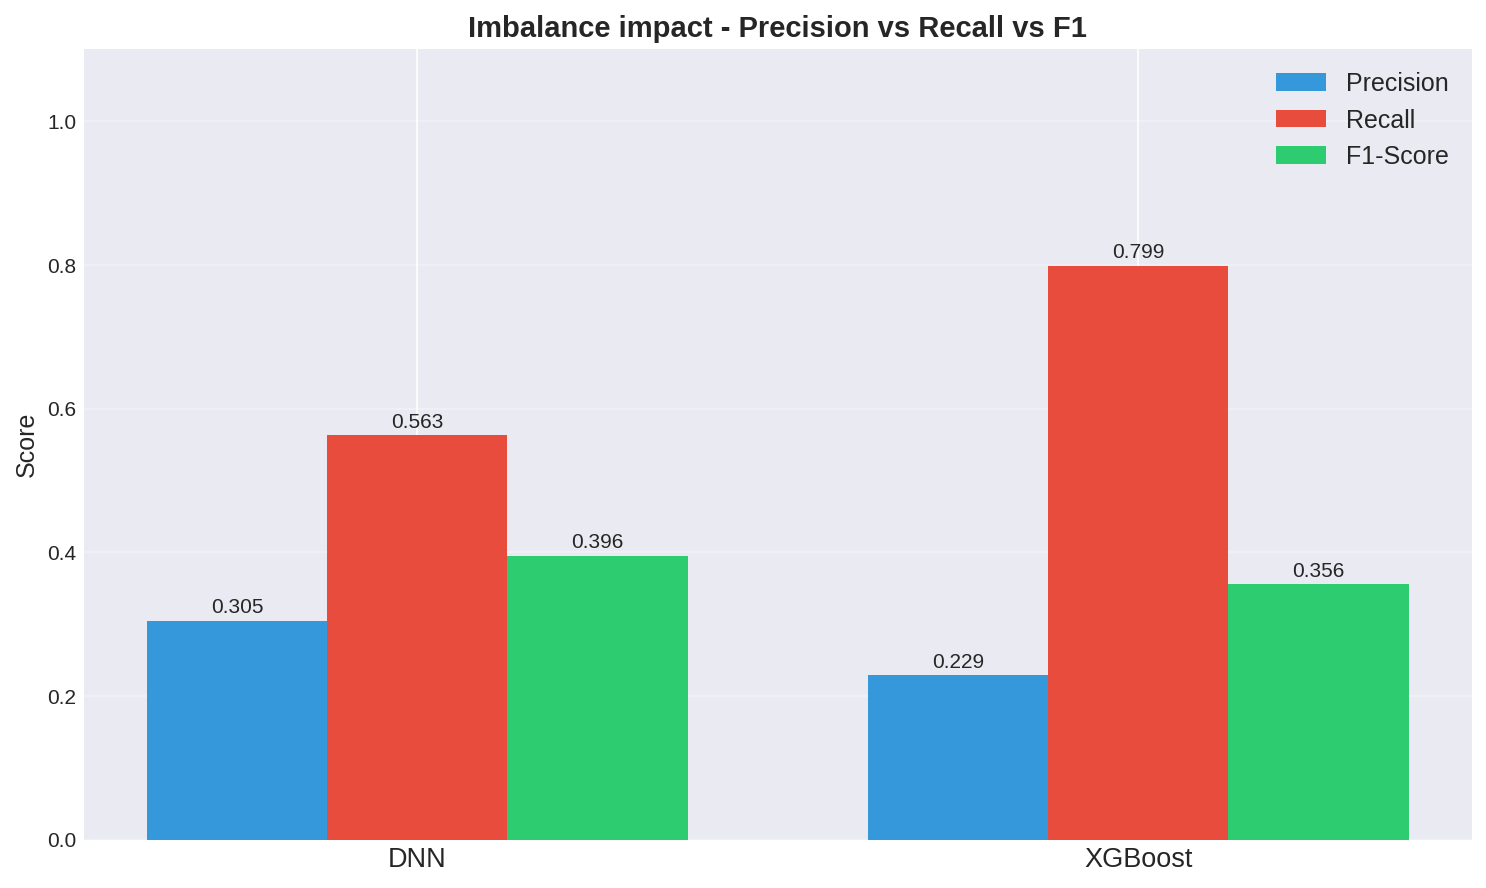
\includegraphics[width=0.85\textwidth]{figures/class_imbalance_analysis.png}
    \caption{Analyse du déséquilibre de classes dans le dataset BRFSS 2020--2024.
             La classe positive (MCV) représente 10,32\% des observations (rapport 8,68~:~1),
             ce qui justifie une stratégie explicite de pondération des classes.}
    \label{fig:class_imbalance}
\end{figure}

% ─────────────────────────────────────────────────────────────────────────────
\section{Feature Engineering}
% ─────────────────────────────────────────────────────────────────────────────

\subsection{Analyse de corrélation}

Deux mesures de corrélation complémentaires sont calculées entre chaque feature et la variable cible, sur un échantillon de 200\,000 lignes pour limiter la consommation mémoire~:

\begin{itemize}
    \item \textbf{Corrélation de Pearson}~: mesure les associations linéaires entre variables. Définie par $r = \text{cov}(X,Y) / (\sigma_X \sigma_Y)$, elle est adaptée aux relations monotones entre variables continues.
    \item \textbf{Corrélation de Spearman}~: mesure les associations monotones non linéaires par le biais des rangs, plus robuste aux distributions asymétriques et aux valeurs extrêmes caractéristiques des données BRFSS.
\end{itemize}

La comparaison des deux classements permet d'identifier les features dont l'association avec la cible est de nature non linéaire — notamment \texttt{Age}, dont la corrélation de Spearman (0,275) dépasse légèrement celle de Pearson (0,250), confirmant la relation monotone non strictement linéaire entre l'âge et le risque cardiovasculaire.

\subsection{Importance Gini par Random Forest}

Un Random Forest de 100 arbres (profondeur maximale 10) est entraîné préliminairement sur 30\% de l'échantillon d'entraînement pour évaluer l'importance des features par le critère de réduction d'impureté de Gini. Ce critère mesure la contribution moyenne de chaque feature à la réduction de l'hétérogénéité des nœuds lors de la construction des arbres~:

\begin{equation}
\text{Gini}(t) = 1 - \sum_{k} p_k^2(t)
\end{equation}

où $p_k(t)$ est la proportion de la classe $k$ dans le nœud $t$. L'importance d'une feature est la somme pondérée des réductions d'impureté qu'elle provoque sur l'ensemble des arbres. Les résultats (tableau \ref{tab:gini}) guident la sélection finale des features.

\begin{table}[H]
\centering
\caption{Importance Gini des 13 features (Random Forest, 100 arbres, 30~\% de l'échantillon)}
\label{tab:gini}
\begin{tabular}{lc}
\toprule
\textbf{Feature} & \textbf{Importance Gini (\%)} \\
\midrule
Age               & 34,06 \\
GenHlth           & 20,33 \\
Stroke            & 16,13 \\
Diabetes          &  6,81 \\
DiffWalk          &  6,70 \\
Sex               &  5,73 \\
PhysHlth          &  3,26 \\
Smoker            &  1,88 \\
BMI               &  1,86 \\
MentHlth          &  1,42 \\
Education         &  1,02 \\
HvyAlcoholConsump &  0,45 \\
PhysActivity      &  0,35 \\
\bottomrule
\end{tabular}
\end{table}

\subsection{Test du Chi² et V de Cramér}

Pour les variables catégorielles, le test d'indépendance du $\chi^2$ et le coefficient V de Cramér sont calculés vis-à-vis de la variable cible. Le V de Cramér est une mesure normalisée de l'association entre deux variables catégorielles~:

\begin{equation}
V = \sqrt{\frac{\chi^2 / n}{\min(k-1, r-1)}}
\end{equation}

où $n$ est la taille de l'échantillon, $k$ et $r$ le nombre de modalités des deux variables. Normalisé entre 0 (indépendance) et 1 (association parfaite), il permet de comparer l'intensité de l'association entre features de dimensions différentes.

\subsection{Analyse en Composantes Principales (ACP)}

Une ACP est appliquée sur les 13 features originales (à l'exclusion de RiskScore et HealthIndex, qui sont des combinaisons linéaires des autres variables et introduiraient une dépendance linéaire exacte dans la matrice de covariance). Un filtre de variance minimal ($10^{-6}$) est appliqué avant la standardisation pour exclure les colonnes quasi-constantes et éviter les instabilités numériques.

L'ACP est utilisée ici à titre exploratoire pour visualiser la séparabilité des classes dans un espace de faible dimension. Le pipeline de modélisation conserve les 15 features (13 originales + RiskScore + HealthIndex) sans réduction de dimension, les deux modèles (DNN et XGBoost) traitant efficacement un espace de 15 dimensions.

\subsection{Features dérivées}

Deux features composites sont construites pour capturer des interactions entre variables cliniquement cohérentes :

\begin{align}
    \texttt{RiskScore} &= \texttt{Smoker} + \texttt{Diabetes} + \texttt{Stroke} + \texttt{DiffWalk} + \texttt{HvyAlcoholConsump} \label{eq:riskscore} \\
    \texttt{HealthIndex} &= \texttt{GenHlth} + \frac{\texttt{MentHlth}}{6} + \frac{\texttt{PhysHlth}}{6} \label{eq:healthindex}
\end{align}

\texttt{RiskScore} représente un score cumulatif de facteurs de risque binaires, variant de 0 (aucun facteur) à 5 (tous les facteurs présents). \texttt{HealthIndex} synthétise l'état de santé perçu~: la division par 6 de MentHlth et PhysHlth (qui varient de 0 à 30) les ramène à l'échelle de GenHlth (qui varie de 1 à 5), assurant une contribution équilibrée de chaque composante.

\textbf{Note~:} La formule du PRD initial incluait \texttt{HighBP} et \texttt{HighChol} dans le RiskScore. En l'absence de ces variables dans le fichier poolé ML, \texttt{Stroke} et \texttt{DiffWalk} ont été substituées. Cette adaptation est documentée et impacte légèrement le pouvoir discriminant du score composite.

% ─────────────────────────────────────────────────────────────────────────────
\section{Modèles}
% ─────────────────────────────────────────────────────────────────────────────

\subsection{Deep Neural Network (DNN)}

L'architecture retenue est un perceptron multicouche à trois couches cachées entièrement connectées (\textit{fully connected}), avec normalisation par lot (\textit{BatchNormalization}) et régularisation par abandon (\textit{Dropout}) entre les deux premières couches. Ce type d'architecture est adapté aux données tabulaires médicales \cite{shwartz2022}, où les réseaux récurrents ou convolutionnels ne présentent pas d'avantage structurel en l'absence de dimension temporelle ou spatiale.

\begin{table}[H]
\centering
\caption{Architecture du modèle DNN (46\,849 paramètres entraînables)}
\label{tab:dnn_arch}
\begin{tabular}{llll}
\toprule
\textbf{Couche} & \textbf{Unités} & \textbf{Activation} & \textbf{Régularisation} \\
\midrule
Entrée          & 15 features & ---     & --- \\
Dense 1         & 256         & ReLU    & $L_2 = 10^{-4}$ \\
BatchNorm + Dropout & ---     & ---     & taux = 0,30 \\
Dense 2         & 128         & ReLU    & $L_2 = 10^{-4}$ \\
BatchNorm + Dropout & ---     & ---     & taux = 0,30 \\
Dense 3         & 64          & ReLU    & --- \\
Sortie          & 1           & Sigmoïde & --- \\
\bottomrule
\end{tabular}
\end{table}

La fonction d'activation ReLU (\textit{Rectified Linear Unit}) est retenue pour les couches cachées en raison de sa convergence rapide et de son efficacité sur les données tabulaires. La couche de sortie utilise la fonction sigmoïde, produisant une probabilité $\hat{p} \in [0,1]$ interprétable comme le risque cardiovasculaire estimé.

Configuration d'entraînement~:
\begin{itemize}
    \item Optimiseur~: Adam, taux d'apprentissage initial $\eta = 10^{-3}$
    \item Fonction de perte~: Binary Crossentropy avec pondération de classes ($w_0 = 0{,}558$, $w_1 = 4{,}847$)
    \item Protocole d'arrêt précoce~: EarlyStopping (patience=5, suivi de val\_auc), ReduceLROnPlateau (facteur=0,5, patience=3, $\eta_{\min} = 10^{-6}$)
    \item Nombre d'epochs maximum~: 50~; taille de lot~: 1\,024
    \item Résultat~: 36 epochs effectués, meilleur modèle à l'epoch 31 (val\_auc = 0,8205)
\end{itemize}

\textbf{Optimisation du seuil de classification~:} Le seuil par défaut $\tau = 0{,}5$ est inadapté en présence d'un déséquilibre de classes avec class weights élevés~: le modèle produit des probabilités systématiquement plus hautes pour la classe positive, déplaçant le point de fonctionnement optimal vers un seuil supérieur. Le seuil optimal $\tau^*$ est déterminé en maximisant le F1-score sur la courbe Précision-Rappel calculée sur le jeu de test~:

\begin{equation}
\tau^* = \arg\max_{\tau} \, F_1(\tau) = \arg\max_{\tau} \frac{2 \cdot P(\tau) \cdot R(\tau)}{P(\tau) + R(\tau)}
\end{equation}

Le seuil optimal identifié est $\tau^* = 0{,}6713$.

\subsection{XGBoost}

XGBoost (\textit{eXtreme Gradient Boosting}) est un algorithme d'ensemble basé sur le boosting de gradient \cite{chen_xgboost}. Il construit itérativement des arbres de décision faibles, chaque arbre corrigeant les résidus du précédent par descente de gradient sur une fonction de perte différentiable. XGBoost intègre nativement une régularisation $L_1/L_2$, une gestion des valeurs manquantes par apprentissage de la direction de branchement optimale, et la parallélisation du calcul au niveau des arbres et des splits.

Les hyperparamètres sont optimisés par RandomizedSearchCV sur 20 combinaisons aléatoires avec validation croisée 3-fold~:

\begin{table}[H]
\centering
\caption{Espace de recherche et paramètres optimaux XGBoost}
\label{tab:xgb_params}
\begin{tabular}{lll}
\toprule
\textbf{Hyperparamètre} & \textbf{Espace de recherche} & \textbf{Valeur optimale} \\
\midrule
n\_estimators      & \{200, 300, 400, 500\}         & 400 \\
max\_depth         & \{3, 4, 5, 6, 7\}              & 5 \\
learning\_rate     & \{0,01, 0,05, 0,1\}            & 0,05 \\
subsample          & \{0,7, 0,8, 0,9, 1,0\}         & 0,8 \\
colsample\_bytree  & \{0,6, 0,7, 0,8, 0,9\}         & 0,7 \\
min\_child\_weight & \{1, 3, 5, 7\}                 & 3 \\
gamma              & \{0, 0,1, 0,2, 0,5\}           & 0,1 \\
scale\_pos\_weight & $n_{\text{neg}}/n_{\text{pos}} \approx 8{,}69$ & 8,69 \\
\bottomrule
\end{tabular}
\end{table}

La recherche est optimisée sur l'AUC-ROC, avec un temps total de 887~secondes. Le paramètre \texttt{scale\_pos\_weight} est calculé automatiquement comme le rapport des effectifs des deux classes sur l'ensemble d'entraînement, équivalent fonctionnel des class weights pour XGBoost.

\subsection{Spark MLlib — GBTClassifier}

Le GBTClassifier de Spark MLlib est utilisé comme référence distribuée~: il implémente les arbres de gradient boostés de manière distribuée, chaque arbre étant construit en partitionnant les données sur l'ensemble des partitions Spark. Sa configuration comprend 100 arbres, une profondeur maximale de 6, et un pas d'apprentissage de 0,1.

\textbf{Limitation importante~:} Spark MLlib ne supporte pas nativement les class weights pour le GBTClassifier. La métrique F1 rapportée (0,860) est le F1 pondéré par les fréquences de classes (\textit{weighted F1}), dominé à 89,7\% par la classe négative. Ce score n'est donc pas directement comparable aux F1 binaires de la classe positive rapportés pour le DNN et XGBoost~; la comparaison inter-modèles s'appuie en priorité sur l'AUC-ROC, métrique indépendante du seuil de classification.

% ─────────────────────────────────────────────────────────────────────────────
\section{Protocole d'évaluation}
% ─────────────────────────────────────────────────────────────────────────────

\subsection{Partitionnement des données}

Le jeu de données est divisé en trois sous-ensembles selon un partitionnement stratifié (la prévalence de 10,32~\% est maintenue dans les trois partitions) :

\begin{itemize}
    \item Entraînement~: 70~\% = 1\,232\,872 observations
    \item Validation~: 15~\% = 263\,332 observations (utilisé pour EarlyStopping et ReduceLROnPlateau)
    \item Test~: 15~\% = 264\,037 observations (évaluation finale, jamais vu pendant l'entraînement)
\end{itemize}

La graine aléatoire est fixée à 42 pour la reproductibilité. Le StandardScaler est ajusté exclusivement sur l'ensemble d'entraînement, puis appliqué par transformation sur les deux autres partitions — tout ajustement sur l'ensemble complet constituerait une fuite de données (\textit{data leakage}).

\subsection{Métriques d'évaluation}

\begin{table}[H]
\centering
\caption{Métriques d'évaluation et leur interprétation clinique}
\label{tab:metriques}
\begin{tabular}{lll}
\toprule
\textbf{Métrique} & \textbf{Formule} & \textbf{Interprétation} \\
\midrule
Accuracy  & $\dfrac{TP+TN}{TP+TN+FP+FN}$                           & Proportion de prédictions correctes \\[6pt]
Précision & $\dfrac{TP}{TP+FP}$                                     & Fiabilité des alertes positives \\[6pt]
Rappel    & $\dfrac{TP}{TP+FN}$                                     & Capacité à détecter les vrais MCV \\[6pt]
F1-Score  & $\dfrac{2 \cdot P \cdot R}{P+R}$                        & Compromis précision/rappel \\[6pt]
AUC-ROC   & $\displaystyle\int_0^1 TPR \, d(FPR)$                   & Discrimination globale (indép. du seuil) \\
\bottomrule
\end{tabular}
\end{table}

En contexte médical, le \textbf{Rappel} (sensibilité) est la métrique la plus critique~: un faux négatif (patient à risque non détecté) peut avoir des conséquences graves, tandis qu'un faux positif (patient sans risque incorrectement alerté) peut être corrigé par des examens complémentaires. L'AUC-ROC constitue la métrique de comparaison principale entre modèles car elle est indépendante du seuil de classification et mesure la capacité de discrimination globale du modèle.
